%http://math.mit.edu/~drew/
%https://math.stackexchange.com/questions/93689/software-for-galois-theory
%SetClassGroupBounds("GRH"); 
%K := QuadraticField(9);
%ClassNumber(K);

%https://en.wikipedia.org/wiki/List_of_triangle_inequalities

\documentclass[12pt, a4paper]{article}
\usepackage[bottom=2cm,top=3cm,left=3cm,right=2cm]{geometry}
\usepackage[utf8]{inputenc}
\usepackage{CJKutf8}
\usepackage{mathtext}
\usepackage{graphicx}
\usepackage{wrapfig}
\usepackage[T1]{fontenc}
\usepackage{blindtext}
\usepackage{tasks}
\usepackage{setspace}
\usepackage{amsmath}
\usepackage{amsfonts}
\usepackage{amssymb}
\usepackage{ wasysym }
\usepackage[portuguese]{babel}
\usepackage[utf8]{inputenc}
\usepackage{mathtext}
\usepackage{graphicx}
\usepackage{wrapfig}
\usepackage[T1]{fontenc}
\usepackage{blindtext}
\usepackage{setspace}
\usepackage{amsmath}
%\usepackage{geometry}
\usepackage{amsthm}
\usepackage{graphics}
%\usepackage{amsfonts}
%\usepackage{lipsum}
\usepackage{amssymb}
\usepackage{CJKutf8} %Pacote para escrever em japonês \begin{CJK}{UTF8}{min} \end{CJK}
\usepackage[portuguese]{babel}
\usepackage{multicol}
% \usepackage{colorspace}
\usepackage{graphicx, color}
\newcommand{\mdc}{{\rm mdc}}
\newcommand{\sen}{{\rm sen}}
\newcommand{\tg}{{\rm tg}}
\newcommand{\cotg}{{\rm cotg}}
\newcommand{\cossec}{{\rm cossec}}
\newcommand{\arctg}{{\rm arctg}}
\newcommand{\arcsen}{{\rm arcsen}}
\newcommand{\pulaquestao}{\newline\newline}
\newcommand{\negrito}[1]{\mbox{\boldmath{$#1$}}} 
\usepackage{pifont}
\newcommand{\heart}{\ensuremath\heartsuit}
\newcommand{\diamonde}{\ensuremath\diamondsuit}
\newtheorem{defi}{Definição}
\newtheorem{propo}{Proposição}
\newtheorem{dem}{Demonstração}
\newtheorem{coro}{Corolário}
\DeclareSymbolFont{extraup}{U}{zavm}{m}{n}
\DeclareMathSymbol{\varheart}{\mathalpha}{extraup}{86}
\DeclareMathSymbol{\vardiamond}{\mathalpha}{extraup}{87}
\setlength{\parindent}{0pt}
\usepackage[framemethod=TikZ]{mdframed}
%\usepackage{lipsum}
\mdfdefinestyle{MyFrame}{%
    linecolor=blue,
    outerlinewidth=2pt,
    roundcorner=20pt,
    innertopmargin=\baselineskip,
    innerbottommargin=\baselineskip,
    innerrightmargin=20pt,
    innerleftmargin=20pt,
    backgroundcolor=white!50!white}
    
%\mdfdefinestyle{Solução}{%
%    linecolor=blue,
%    outerlinewidth=1pt,
%    roundcorner=8pt,
%    innertopmargin=4pt%\baselineskip,
%    innerbottommargin=0pt%\baselineskip,
%    innerrightmargin=20pt,
%    innerleftmargin=20pt,
%    backgroundcolor=white!50!white}
    
    
    \mdfdefinestyle{DAS}{%
    linecolor=blue,
    outerlinewidth=2pt,
    roundcorner=20pt,
    innertopmargin=\baselineskip,
    innerbottommargin=\baselineskip,
    innerrightmargin=20pt,
    innerleftmargin=20pt,
    backgroundcolor=white!50!green}
% \definespotcolor{mygreen}{PANTONE 7716 C}{.83, 0, .00, .51}
% \definespotcolor{tuti}{}{0.6, 0, 1, .508}
\title{PIC - Programa de Iniciação Científica}
\author{Douglas de Araujo Smigly}
\date{}
\begin{document}
\definecolor{Floresta}{rgb}{0.13,0.54,0.13}
\maketitle
\begin{center}
\large\textbf{\textcolor{Floresta}{Ciclo 1 - Encontro 1 - Álgebra}}\\
\end{center}
%\begin{multicols*}{2}
%\setlength{\columnseprule}{0.78pt}
%\raggedcolumns
%\columnbreak
\textcolor{blue}{\bf(1)} Se $a - b = 1$ e $ab = 1,$ qual é o valor de $a^2 + b^2?$
\newline\newline
\textcolor{blue}{\bf(2)} (OBMEP 2010) Na figura, $x$ é a média aritmética dos números que estão nos círculos claros e $y$ é a média aritmética dos números que estão nos círculos escuros. Quais são os valores de $x$ e $y$?

\begin{figure}[!h]
    \centering
    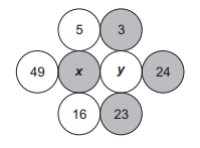
\includegraphics{Figuras/ex2enc1.png}
\end{figure}

\textcolor{blue}{\bf(3) $\varheart$} Observe que na figura da questão anterior temos que $5 \cdot 3 + 1 = 16$ e $ 5 \cdot 3 + 5 + 3 = 23.$ Além disso, $24 = 23 + 1$ e $49 = 24 \cdot 2 + 1.$ Considere de forma genérica $a$ e $b$ dois números naturais positivos com os números descritos na figura abaixo, com $c = ab + 1, d = ab + a + b,$ $e = 2(d+1)+1$ e $x$ e $y$ como na questão anterior.
\begin{figure}[!h]
    \centering
    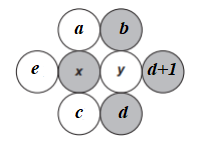
\includegraphics{Listas do PIC/varex2enc1.png}
\end{figure}
Se a diferença entre $a$ e $b$ é $k,$ para que valores de $k$  $x$ e $y$ são números naturais? Será que existem infinitos valores de $a$ e $b$ tais que $x$ e $y$ são quadrados perfeitos?
\newline \newline
\textcolor{blue}{\bf(4)} (Banco de Questões - OBMEP 2010) Na figura, o número $8$ foi obtido somando-se dois números diretamente abaixo de sua casa. Fazendo-se o mesmo para preencher as casas em branco, obtém-se o $42$ na casa indicada. Qual é o valor de $x?$
\begin{figure}[!h]
    \centering
    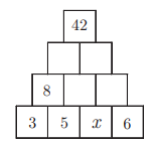
\includegraphics{Listas do PIC/2encontro1ciclo1.png}
\end{figure}
\newpage
\textcolor{blue}{\bf(5)} (Banco de Questões - OBMEP 2010) Sendo $x > 0,$ $y > 0,$ $x > y$ e $z \neq 0,$ encontre a única desigualdade falsa entre as desigualdades abaixo.
\begin{tasks}[counter-format={(tsk[a])},label-width=3.6ex, label-format = {\bfseries}, column-sep = {0pt}](5)
\task[\textcolor{Floresta}{$\negrito{(a)} $}] $x + z > y + z$
\task[\textcolor{Floresta}{$\negrito{(b)} $}] $x - z > y - z$
\task[\textcolor{Floresta}{$\negrito{(c)} $}] $xz > yz$
\task[\textcolor{Floresta}{$\negrito{(d)} $}] $\dfrac{x}{z^2} > \dfrac{y}{z^2}$
\task[\textcolor{Floresta}{$\negrito{(e)} $}] $xz^2 > yz^2$
\end{tasks}
\textcolor{blue}{\bf(6)} (Banco de Questões - OBMEP 2013 - Adaptada) No interior de cada um dos círculos que aparecem na figura abaixo, a pequena Luana colocou os números $1,2,3,4,5,6$ e $7.$
\begin{figure}[!h]
    \centering
    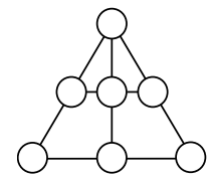
\includegraphics{Listas do PIC/5encontro1ciclo1.png}
\end{figure}





Ela o fez de modo que todos os números foram usados. O seu irmão mais velho, Pedro, olhou para cada trio de círculos colineares e somou os três números neles colocados. Pedro observou que a soma resultava ser sempre a mesma.
\begin{tasks}[counter-format={(tsk[a])},label-width=3.6ex, label-format = {\bfseries}, column-sep = {0pt}](1)
\task[\textcolor{Floresta}{$\negrito{(a)} $}] Mostre que o número colocado por Luana no círculo do topo é $4$ e que a soma constante observada por Pedro é igual a $12.$
\task[\textcolor{Floresta}{$\negrito{(b)} $}] Encontre uma maneira pela qual Luana poderia ter conseguido realizar tal proeza.
\task[\textcolor{Floresta}{$\negrito{(c)} \varheart$}] \ \ \ \ Luana obteve uma figura com quatro duplicatas da primeira, desta vez colocando os números de $1$ a $25$, de modo que as mesmas regras anteriores fossem respeitadas em cada triângulo. Pedro conseguirá fazer a mesma observação que anteriormente?
\end{tasks}
\begin{figure}[!h]
    \centering
    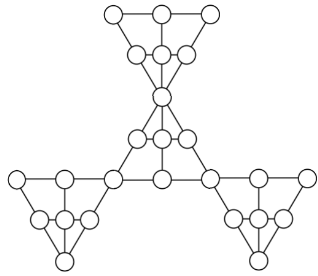
\includegraphics[scale=0.54]{Listas do PIC/var8encontro1ciclo1.png}
\end{figure}
\textcolor{blue}{\bf(7)} (OBMEP 2013) O número de alunos matriculados na Escola Municipal de Pirajuba permaneceu o mesmo nos anos de $2011$ a $2013.$ Em $2012,$ foram construídas $5$ novas salas de aula e,
com isso, a média de alunos por sala foi reduzida em $6$ alunos em relação à média de
$2011.$ Em $2013,$ foram construídas mais $5$ salas de aula e, com isso, a média de alunos
por sala foi reduzida em $5$ alunos em relação à média de $2012.$ Quantos alunos tem a
Escola Municipal de Pirajuba?
\newline\newline
\textcolor{blue}{\bf(8)} (OBMEP 2006) A figura representa parte de uma régua graduada de meio em meio centímetro, onde estão marcados alguns pontos. Qual deles melhor representa o número $2x - 2?$
\begin{figure}[!h]
    \centering
    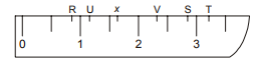
\includegraphics{Listas do PIC/8encontro1ciclo1.png}
\end{figure}

\textcolor{blue}{\bf(9)} (FGV) Uma fábrica de camisas tem um custo mensal de operação dado por $C = 5000 + 15x,$ onde $x$ é o número de camisas produzidas por mês. Cada camisa é vendida por
$R\$ 25, 00$ e, atualmente, o lucro mensal da fábrica é de $R\$ 2000, 00.$ Para dobrar esse
lucro, a fábrica deverá produzir e vender mensalmente:
\begin{tasks}[counter-format={(tsk[a])},label-width=3.6ex, label-format = {\bfseries}, column-sep = {0pt}](1)
\task[\textcolor{Floresta}{$\negrito{(a)} $}] o dobro do que produz e vende hoje.
\task[\textcolor{Floresta}{$\negrito{(b)} $}] $100$ unidades a mais do que produz e vende hoje.
\task[\textcolor{Floresta}{$\negrito{(c)} $}] $200$ unidades a mais do que produz e vende hoje.
\task[\textcolor{Floresta}{$\negrito{(d)} $}] $300$ unidades a mais do que produz e vende hoje.
\task[\textcolor{Floresta}{$\negrito{(e)} $}] $50\%$ a mais do que produz e vende hoje.
\end{tasks}
\textcolor{blue}{\bf(10)} (ENEM 2013) Na aferição de um novo semáforo, os tempos são ajustados de modo que, em cada ciclo completo (verde-amarelo-vermelho), a luz amarela permaneça acesa por $5$ segundos, e o tempo em que a luz verde permaneça acesa seja igual a $\frac{2}{3}$ do tempo em que a luz vermelha fique acesa. Sabe-se que cada ciclo dura $Y$segundos e, nele, a luz
verde fica acesa durante $X$ segundos. Qual das expressões a seguir representa a
relação entre $X$ e $Y$?

\begin{tasks}[counter-format={(tsk[a])},label-width=3.6ex, label-format = {\bfseries}, column-sep = {0pt}](1)
\task[\textcolor{Floresta}{$\negrito{(a)} $}] $5X - 3Y + 15 = 0.$
\task[\textcolor{Floresta}{$\negrito{(b)} $}] $5X - 2Y + 10 = 0.$
\task[\textcolor{Floresta}{$\negrito{(c)} $}] $3X - 3X + 15 = 0.$
\task[\textcolor{Floresta}{$\negrito{(d)} $}] $3X-2Y+15 = 0.$
\task[\textcolor{Floresta}{$\negrito{(e)} $}] $3X - 2Y + 10 = 0.$
\end{tasks}
\textcolor{blue}{\bf(11)} (OBM 2013) Os gatos Mate e Tica estão dormindo no sofá. Mate chegou antes e, quando Tica chegou, ela ocupou um quarto da superfície que havia sobrado do sofá. Os dois gatos
juntos ocupam exatamente a metade da superfície do sofá. Qual porção da superfície do sofá está ocupada por Tica?
\newline
\newline
\textcolor{blue}{\bf(12)} Uma empresa possui $500$ toneladas de grãos em seu armazém e precisa transportá-los a um cliente. O transporte pode ser feito por caminhões ou por trem. Para cada
tonelada transportada por trem paga-se $R\$ 8,00$ de custo fixo e $R\$ 0,015$ por
quilômetro rodado. O transporte rodoviário exige $25$ caminhões. Para cada caminhão
utilizado paga-se $R\$ 125,00$ de custo fixo, além de $R\$ 0,50$ por quilômetro rodado.
Suponha que $x$ seja a distância, em quilômetros, entre o armazém e o cliente. Para que
intervalo de variação de $x$ o transporte por trem é mais vantajoso do que o transporte
por caminhões?
\newline\newline
\textcolor{blue}{\bf(13) $\varheart$} Seja $x$ um número real tal que $x + \dfrac{1}{x} = 3.$ Quanto vale $x^2 + \dfrac{1}{x^2}?$ É possível encontrar uma fórmula para calcular $x^n + \dfrac{1}{x^n},$ onde $n \in \mathbb{N}?$
%https://artofproblemsolving.com/community/c6h473647p2651848
\newline\newline
\textcolor{blue}{\bf(14) $\varheart$} O valor de
\[
199919981997^2 - 2 \cdot 199919981994^2 + 199919981991^2
\]
é igual a
\begin{tasks}[counter-format={(tsk[a])},label-width=3.6ex, label-format = {\bfseries}, column-sep = {0pt}](5)
\task[\textcolor{Floresta}{$\negrito{(a)} $}] $12$
\task[\textcolor{Floresta}{$\negrito{(b)} $}] $14$ 
\task[\textcolor{Floresta}{$\negrito{(c)} $}] $16$
\task[\textcolor{Floresta}{$\negrito{(d)} $}] $18$
\task[\textcolor{Floresta}{$\negrito{(e)} $}] $20$
\end{tasks}
\textcolor{blue}{\bf(15) $\varheart$} Se $a$ e $b$ são números reais positivos, mostre que
\[
4(a^3 + b^3) \ge (a+b)^3
\]
\newline\newline
\textcolor{blue}{\bf(16) $\varheart$} Uma fábrica de camisas tem um custo mensal de operação dado por $C = 5000 + 15x$, onde $x$ é o número de camisas produzidas por mês. Cada camisa é vendida por $R\$ 25,00$ e, atualmente, o lucro mensal da fábrica é de $R\$ 2000,00.$  Para dobrar esse lucro, quantas camisas a fábrica deverá produzir e vender mensalmente?
\newline\newline
\textcolor{blue}{\bf(17) $\varheart$} (IMO 1960) Encontre os valores de $x$ para os quais a seguinte desigualdade é válida:
\[
\left(\frac{2x}{(1 - \sqrt{1 + 2x})}\right)^2 < 2x + 9
\]
\textcolor{white}{Oi}
\newline \newline
Exercícios marcados com $\varheart$ são extras.
\end{document}
SetClassGroupBounds("GRH"); 
K := QuadraticField(9);
ClassNumber(K);
Q := PolynomialRing(GF(2), 2);
Q;
K := QuadraticField();
G := GaloisGroup(K);
G;
\begin{CJK}{UTF8}{min}
露の世は 露の世ながら さりながら当時では老人と呼べる50歳代半ばでようやく授かったわが子への愛とその突然死を伝えた「露の世」のくだりは、その日記体句文集「おらが春」のクライマックスとなっています。

5月には数え二歳の誕生を迎えて詠んだ句に、
「這へ笑へ二つになるぞけさからは」と喜びを謳歌したばかり。

それが、翌6月にはもはや草葉の陰へと、その露の朝日に立ちどころに消えるごとく、儚くも身罷ってしまったとは。

人の世は朝露の如く無常なのだと、悔みを述べ慰問するあの人、この人。さは「さりながら」…それは確かにそうなのだけれども。
いかに「あきらめ顔しても、思い切りがたきは、恩愛のきづな也けり。」と、わが心中は耐えきれず切々と泣き崩れるばかり。わが子「さと」女を思う「大切」はやがて「あなた任せ」の境地へと通じていくものでしょう。
\end{CJK}